\section{Hunt-Editor Web-App}

\subsection{Übersicht}

Über den Hunt-Editor kann der Organisator Schnitzeljagden verwalten. Hierzu startet er die Anwendung und landet auf die Dashboard-Ansicht. Hier erhält er eine Übersicht von erstellten Schnitzeljagden. Ihm wird die Funktionalität zur Erstellung (\textit{Create}) angeboten. Er kann Titel und Beschreibung sowie die jeweiligen Aufgaben mit Hinweis und Lösung anlegen und speichern. Die Reihenfolge der Reihenfolge der Aufgaben kann bearbeitet werden.

\subsection{Wireframing}

Um den Editor zu entwickeln, der das Anlegen und Verwalten von Schnitzeljagden ermöglicht, wurde zunächst der Ansatz des Wireframings verwendet. Wireframing ist eine wesentliche Phase im Designprozess, die es ermöglicht, die Struktur und Funktionalität einer Anwendung visuell darzustellen, bevor detaillierte Design- und Entwicklungsarbeiten beginnen. In dieser frühen Planungsphase wird ein einfaches, oft schematisches Layout der Benutzeroberfläche erstellt, das die Anordnung der verschiedenen Elemente wie Buttons, Menüs, und interaktiven Komponenten zeigt.

Im Folgenden werden die verschiedenen Wireframes aufgezeigt und erläutert, wieso sie eine solide Grundlage für die weitere Entwicklung des Editors boten, welche Stärken sie in Bezug auf Benutzerfreundlichkeit und Funktionalität aufwiesen, und welche Schwächen oder Herausforderungen während der Umsetzung erkannt wurden, die in späteren Phasen berücksichtigt werden mussten.

\begin{figure}[H]
  \centering
  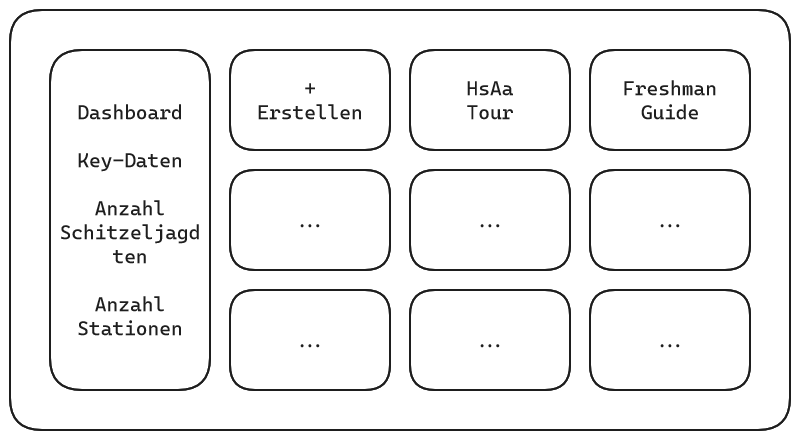
\includegraphics[width=1\textwidth]{images/wireframing/PrAr_Scavhunt_Wireframing-2.1.png}
  \caption{Skizze Dashboard des Hunt-Editors}
  \label{fig:wireframing-frontend-hunt-editor-3}
\end{figure}

Dies war ein Wireframe, was relativ am Anfang der Entwicklungsphase entstanden ist. Hier wurde auf ein Grid-Layout gesetzt, um die Schnitzeljagden anzuzeigen. An der Seite befindet sich eine Sidebar, in der verschiedene Key-Daten abgelesen werden können. Da es aber durch Architekturänderungen keine Stationen mehr gibt, fällt diese Information weg. Das Grid-Layout sollte aber bestehen bleiben.

\begin{figure}[H]
  \centering
  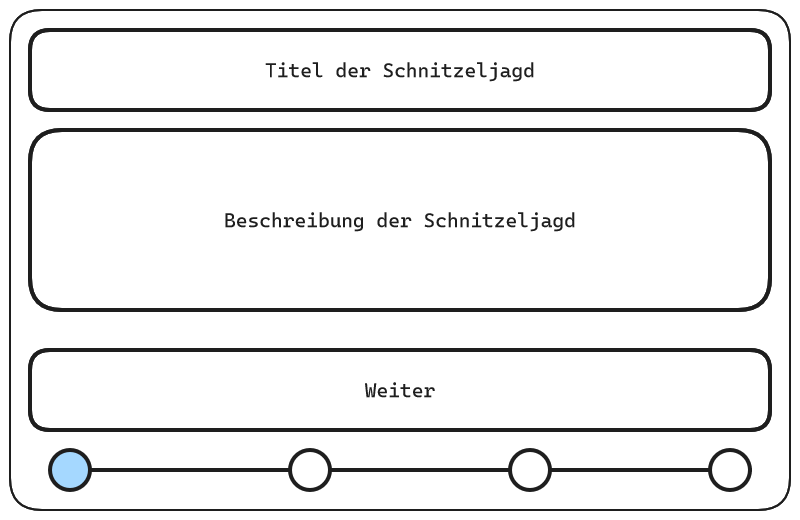
\includegraphics[width=1\textwidth]{images/wireframing/PrAr_Scavhunt_Wireframing-2.2.png}
  \caption{Skizze für Eingabe von Basisdaten im Hunt-Editor}
  \label{fig:wireframing-frontend-hunt-editor-4}
\end{figure}

Hier wird nun der Prozess des Erstellen einer Schnitzeljagd beschrieben, gefallen hat uns hier das Verwenden einer Progressbar, um den aktuellen Fortschritt beim Erstellen anzuzeigen. Auch die Eingabe von Titel und Beschreibung sollte so später übernommen werden. 

\begin{figure}[H]
  \centering
  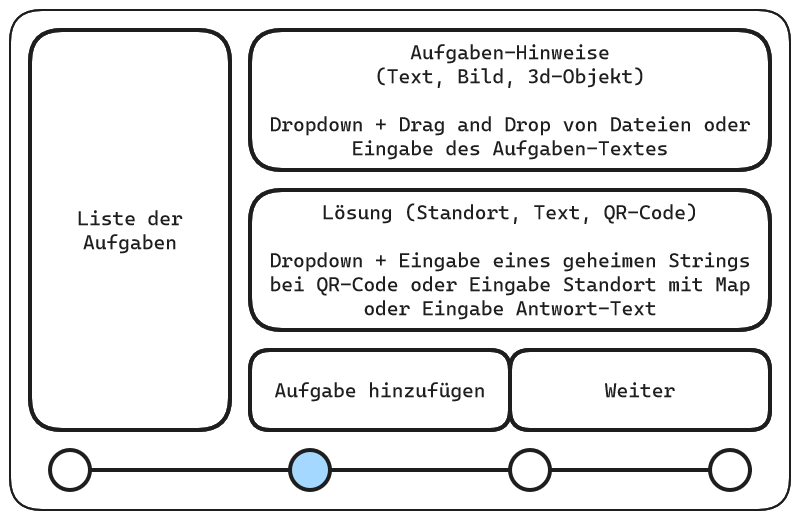
\includegraphics[width=1\textwidth]{images/wireframing/PrAr_Scavhunt_Wireframing-2.3.png}
  \caption{Skizze für Anlegen von Aufgaben im Hunt-Editor}
  \label{fig:wireframing-frontend-hunt-editor-5}
\end{figure}

Nun zum schwersten Teil, das Anlegen und Bearbeiten von Aufgaben in einer Schnitzeljagd. Hier war zunächst der Ansatz, auf der linken Seite eine Tabelle der Aufgaben zu führen. Durch Klick auf die entsprechende Zeile werden dann auf der rechten Seite die Aufgabe und Lösung angezeigt. Hier ist auch noch der Aufgabentyp "3d-Objekt" vorhanden, welcher am Schluss nicht übernommen wurde. 

\begin{figure}[H]
  \centering
  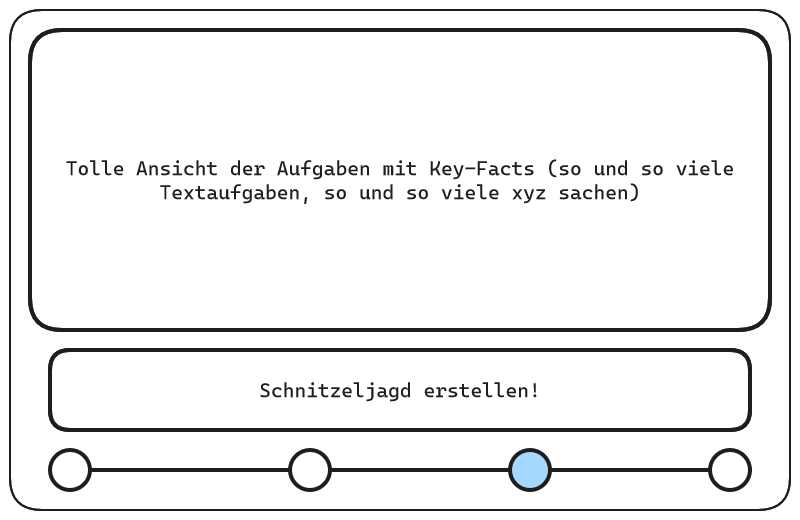
\includegraphics[width=1\textwidth]{images/wireframing/PrAr_Scavhunt_Wireframing-2.4.png}
  \caption{Skizze zur Übersicht einer Schnitzeljagd im Hunt-Editor}
  \label{fig:wireframing-frontend-hunt-editor-6}
\end{figure}

Dieses Wireframe zeigt zum Schluss nochmal eine Übersicht aller wichtigen Infos der Schnitzeljagd an. Dieses Konzept hat uns gut gefallen. 

\begin{figure}[H]
  \centering
  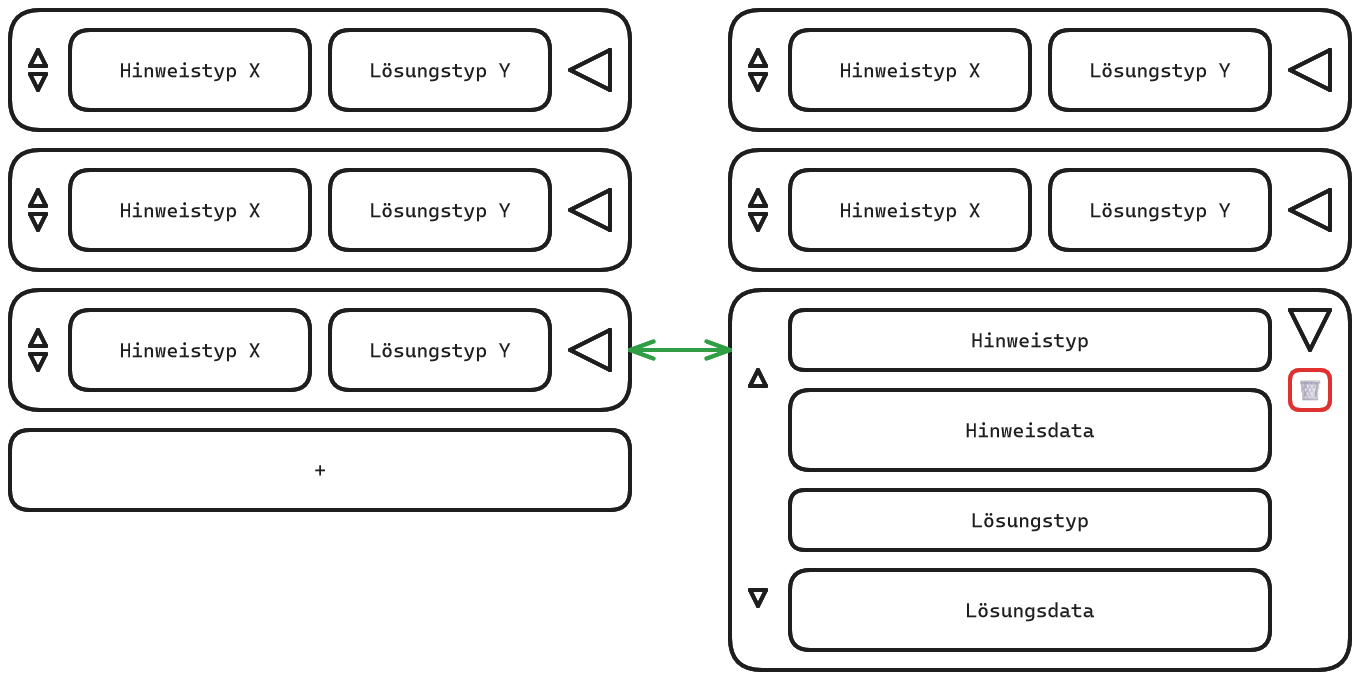
\includegraphics[width=1\textwidth]{images/wireframing/PrAr_Scavhunt_Wireframing-3.png}
  \caption{Skizze zur Auflistung von Aufgaben im Hunt-Editor}
  \label{fig:wireframing-frontend-hunt-editor-7}
\end{figure}

Da die seitliche Liste aus Abbildung \ref{fig:wireframing-frontend-hunt-editor-5} zum Anzeigen der Aufgaben für mobile Geräte ungeeignet ist, haben wir uns für den Ansatz aus Abbildung \ref{fig:wireframing-frontend-hunt-editor-7} entschieden. Hier werden die Aufgaben nacheinander angezeigt und deren Reihenfolgen kann über das Bedienen der Pfeiltasten angepasst werden. Um die Aufgaben zu bearbeiten, können diese über den Button auf der rechten Seite aufgeklappt und wieder zugeklappt werden. Im aufgeklappten Zustand befindet sich jeweils ein Dropdown für Aufgabe und Lösung als auch Eingabefelder / FileUpload oder eine Map Integration für Standort als Lösung. 

\section{Participant Web-App}

\subsection{Übersicht}

Über die Participant Web-App kann sich ein Teilnehmer an einer Schnitzeljagd anmelden. Hierzu startet er die Anwendung und landet auf einer Begrüßungsseite. Hier kann er sehen, wie viele Teilnehmer und wie viele Teilnahmen es insgesamt gibt. Um nun einer Schnitzeljagd beizutreten, kann der Teilnehmer einem Organisator eine Mail schreiben. Erhält er daraufhin einen Einladungslink für eine Schnitzeljagd, so muss er dort nur einen Nutzernamen und ein Passwort auswählen. Mit diesem Nutzernamen und Passwort meldet er sich im in Kapitel \ref{subsec:swentwurf:hunt-game} beschriebenen Hunt-Game an.

\subsection{Wireframing}
% TODO: bissle Wireframing nachholen und hier rein

\section{Hunt-Game Web-App} \label{subsec:swentwurf:hunt-game}

\subsection{Übersicht}
Beim Start der Anwendung sieht der Teilnehmer eine Sammlung an Bildern der Hochschule Aalen, darunter befindet sich eine kleine Timeline, die den Entwicklungsprozess der Projektarbeit beschreibt. Um an einer Schnitzeljagd teilnehmen zu können, muss sich der Teilnehmer mit dem gewählten Nutzernamen und Passwort aus der Participant Web-App anmelden. Daraufhin wird ihm eine Übersicht von allen Schnitzeljagden angezeigt, für welche er sich registriert hat. Hier wird in \textit{Ongoing, Complete} und \textit{Expired} unterschieden, dies wird durch den ParticipationStatus ermittelt. Wählt er eine valide Schnitzeljagd aus, so startet der Spielablauf. 

\subsection{Spielablauf} \label{cha:swentwurf:spielablauf}

Abbildung \ref{fig:hunt_game_spielablauf} stellt den Spielablauf als UML-Programmablaufplan dar. 

\begin{figure}[H]
  \centering
  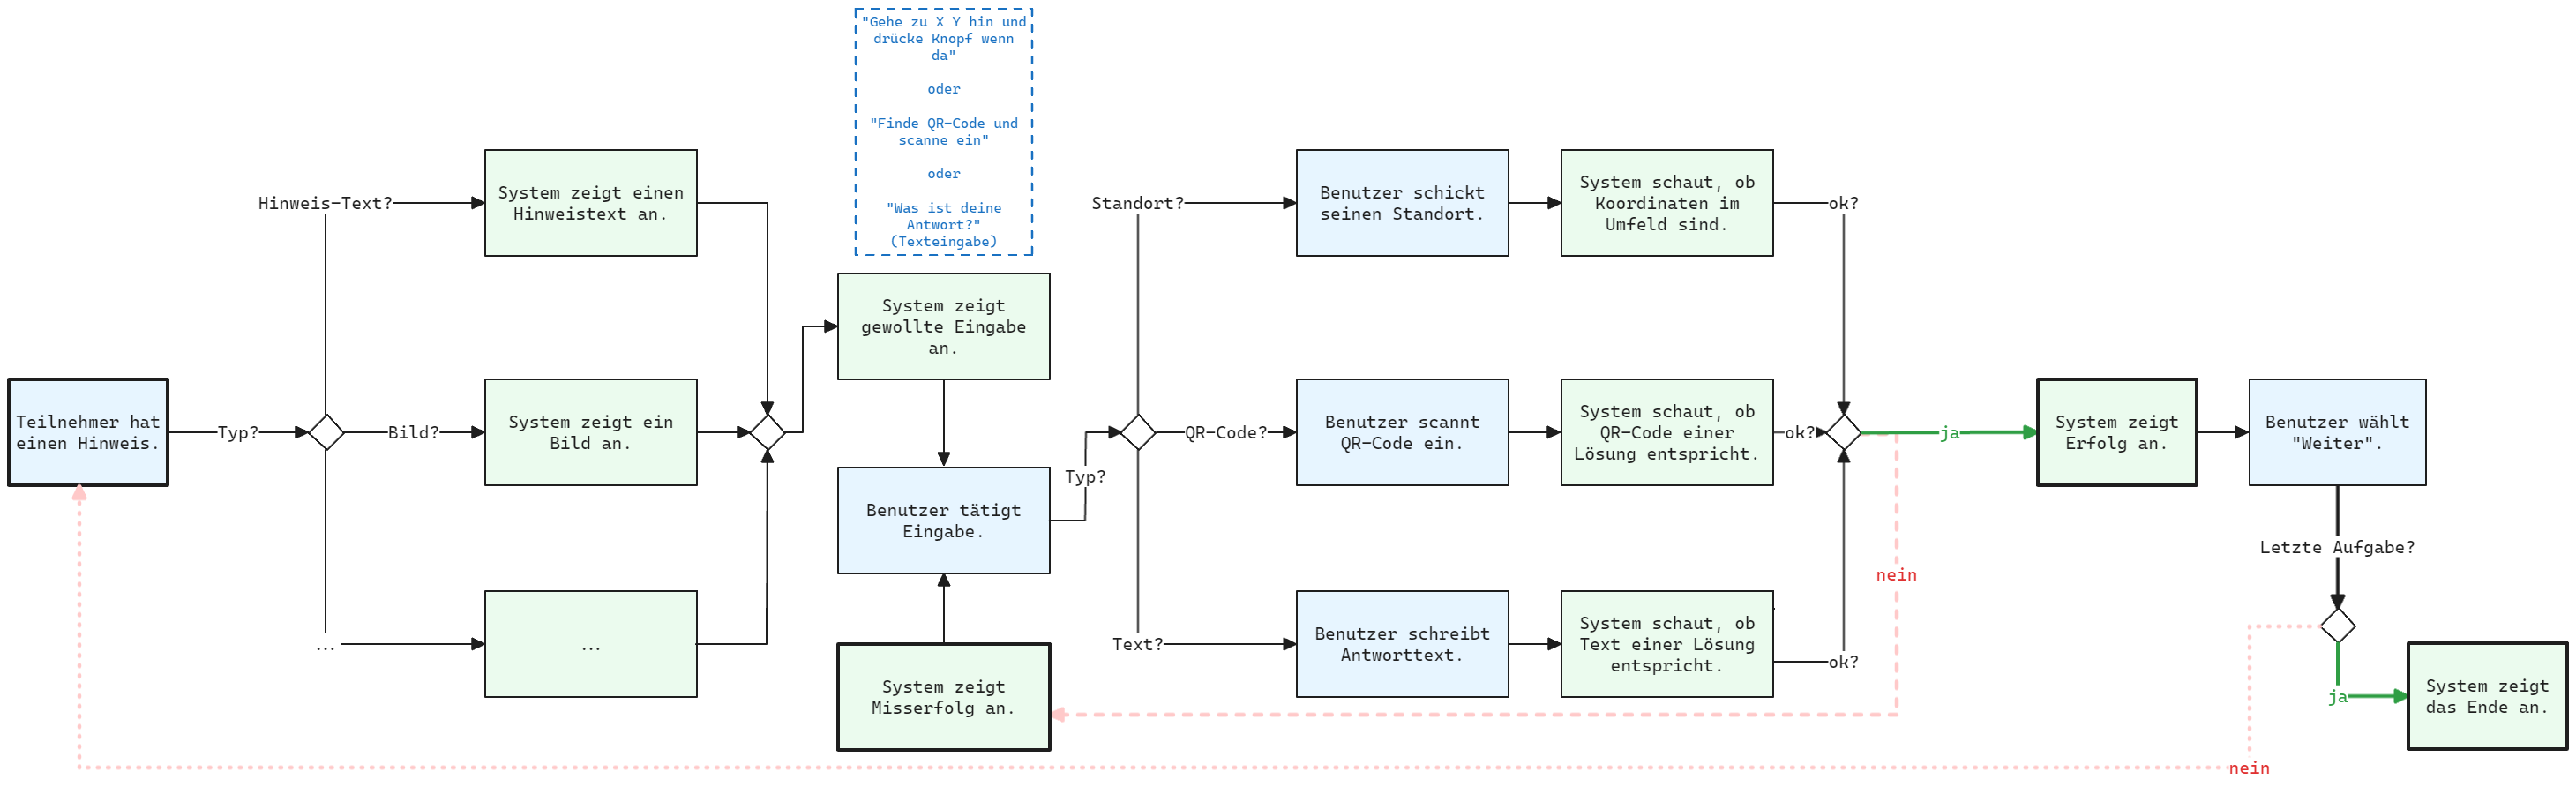
\includegraphics[width=\textwidth]{images/PrAr_Spielablauf.png}
  \caption{Skizze Spielablauf als UML-Programmablaufplan}
  \label{fig:hunt_game_spielablauf}
\end{figure}

Nachdem der Teilnehmer eine valide Schnitzeljagd ausgewählt hat, beginnt der eigentliche Spielablauf. Zu Beginn wird dem Teilnehmer der aktuelle Hinweis präsentiert, der ihn zur nächsten Station oder Aufgabe führen soll. Die Hinweise sind in zwei Typen unterteilt: Text und Bild. Bei einem Text-Hinweis wird dem Teilnehmer ein beschreibender Text angezeigt, der Informationen oder Anweisungen zur nächsten Station enthält. Bei einem Bild-Hinweis wird stattdessen ein Bild angezeigt, das visuelle Hinweise oder Details enthält, die zur Lösung der Aufgabe beitragen.

Unter dem Hinweis befindet sich ein Button, über den der Teilnehmer seine Lösung einreichen kann. Hierbei gibt es drei verschiedene Lösungstypen, die je nach Aufgabe variieren:
\begin{itemize}
    \item \textbf{Textlösung}: Der Teilnehmer gibt seine Lösung in ein Textfeld ein. Dies kann beispielsweise ein gesuchtes Wort, ein Satz oder eine Zahlenkombination sein.

    \item \textbf{QR-Code}: Bei Aufgaben, die einen QR-Code erfordern, wird die Kamera des Geräts aktiviert, um den QR-Code zu scannen. Dieser QR-Code kann an verschiedenen Orten versteckt sein und enthält die notwendigen Informationen oder Anweisungen, um zum nächsten Hinweis zu gelangen.

    \item \textbf{Location}: Wenn die Lösung in Form eines geografischen Standorts vorliegen soll, wird der Teilnehmer aufgefordert, den Standortzugriff zu erlauben. Der Browser ermittelt dann die aktuellen GPS-Koordinaten des Geräts und überprüft, ob diese mit der erwarteten Lösung übereinstimmen.
\end{itemize}

Der Spielablauf wiederholt sich, bis alle Aufgaben gelöst sind. Bei den Lösungstypen Text und Location erhält der Teilnehmer zusätzlich Hinweise, falls seine Lösung nicht korrekt ist. Diese Hinweise geben an, dass die Lösung fast richtig ist, aber noch Anpassungen erfordert. Dies dient dazu, die Teilnehmer zu ermutigen und ihnen eine Chance zu geben, ihre Antwort zu verbessern.




